\mathbb{R} \documentclass{article}


\usepackage{fancyhdr}
\usepackage{extramarks}
\usepackage{amsmath}
\usepackage{amsthm}
\usepackage{amsfonts}
\usepackage{tikz}
\usepackage[plain]{algorithm}
\usepackage{algpseudocode}
\usepackage{enumerate}
\usepackage{tikz}
\usepackage{listings}
\usepackage{hyperref}
\usepackage{subfigure}
\usepackage[graphicx]{realboxes}
\usepackage{xcolor}
\usepackage{color}



% 代码块高级设置
\lstset{
% basicstyle=\footnotesize,                 % 设置整体的字体大小
showstringspaces=false,                     % 不显示字符串中的空格
frame=single,                               % 设置代码块边框
numbers=left,                               % 在左侧显示行号
% numberstyle=\footnotesize\color{gray},    % 设置行号格式
numberstyle=\color{darkgray},               % 设置行号格式
backgroundcolor=\color{white},              % 设置背景颜色
keywordstyle=\color{blue},                  % 设置关键字颜色
commentstyle=\it\color[RGB]{0,100,0},       % 设置代码注释的格式
stringstyle=\sl\color{red},                 % 设置字符串格式
}

\hypersetup{hidelinks,
	colorlinks=true,
	allcolors=black,
	pdfstartview=Fit,
	breaklinks=true}

%
% Basic Document Settings
%  

\topmargin=-0.45in
\evensidemargin=0in
\oddsidemargin=0in
\textwidth=6.5in
\textheight=9.0in
\headsep=0.25in

\linespread{1.1}

\pagestyle{fancy}
\lhead{}
\chead{\hmwkClass : \hmwkTitle}
\rhead{\firstxmark}
\lfoot{\lastxmark}
\cfoot{\thepage}

\renewcommand\headrulewidth{0.4pt}
\renewcommand\footrulewidth{0.4pt}

\setlength\parindent{0pt}



%
% Homework Details
%   - Title
%   - Due date
%   - Class
%   - Instructor
%   - Class number
%   - Name
%   - Student ID

\newcommand{\hmwkTitle}{Lab 3 Report}
\newcommand{\hmwkDueDate}{Dec 1st}
\newcommand{\hmwkClass}{Advanced Computer Architecture}
\newcommand{\hmwkClassInstructor}{Professor Chundong Wang}

% 正式选课名单确定之后,根据通知填写所在班级编号

\newcommand{\hmwkAuthorName}{Zhenghong Yu}
\newcommand{\hmwkAuthorMail}{yuzhh1@shanghaitech.edu.cn}
\newcommand{\hmwkAuthorID}{2020533156}


%
% Title Page
%

\title{
    \vspace{2in}
    \textmd{\textbf{\hmwkClass:\\  \hmwkTitle}}\\
    \normalsize\vspace{0.1in}\small{Due\ on\ \hmwkDueDate\ at 11:59am}\\
   \vspace{2in}
}

\author{
	Name: \textbf{\hmwkAuthorName} \\
    Mailbox: \textbf{\hmwkAuthorMail} \\
	Student ID: \hmwkAuthorID}
\date{}

\renewcommand{\part}[1]{\textbf{\large Part \Alph{partCounter}}\stepcounter{partCounter}\\}

\begin{document}

\maketitle
\pagebreak
\tableofcontents

\pagebreak


\subsection{Preknowledge}
\textcolor[rgb]{1,0,0}{\textbf{You should read following carefully, since they are very important to Lab3 implementation}}\\
The Lab2 is implemented in the branch \textbf{Lab3}, both tasks(Task1, Task2) are all realized in this branch.\\
To specify two cores, you may follow:
\begin{itemize}
  \item For all task input, the format should be like: \textbf{./Simulator -c0 example1.riscv -c1 example2.riscv} as showed in Lab3 pdf. You must specify two programs of two core(e.t. you can't let one core to be idle). Also, I do not support other format like \textbf{-b} or something else. The branch predict policy is NT in default. 
  \item The \textbf{CMakeLists.txt} is rewrite and do not support complier \textbf{CacheSim} and \textbf{CacheOptimized} anymore, please do not change the \textbf{CMakeLists.txt}
\end{itemize} 
To gain more readable ouput, I change \textbf{fprintf()} to \textbf{sprintf()} to some special char pointer variables(e.t. \textbf{core0\_out, core1\_out}), and after two threads finished, I print these variables out(e.t. \textbf{putsline()}). However, the running comments of shared memory operations is still using \textbf{fprintf()} since they are strictly synchronized, they should be quite readable and beautiful.\\
The l1, l2, l3, memory cache line size should all be same and fixed as 32, do not change it.\\
Due to some strange reason, it rarely (I meet in about only 1 times and I cant repreduction it) will crashed and result in read invalid byte, however the address should be valid. If you run into this situation, just ignore it and rerun program.

\section{Task1: Two threads Simulator}
\subsection{Requirement}
\begin{itemize}
  \item Two cores. Different program different core. Own registers, PC, piplines, two-level private caches. Shared L3 cache, memory. 
  \item Avoid conflict between two programs' address.
\end{itemize} 
\subsection{Implementation}
\subsubsection{How to begin run two threads?}
It is common to use \textbf{pthread.h} lib to help me do multi thread single program work. I take core 0 to thread 0 and take core 1 to thread 1. The two thread almost own private class and variable except memory, l3cache, some assist global variables. Here is some global definition in \textbf{MainCPU.cpp}
\begin{lstlisting}[language=c++]
char *elfFile0 = nullptr; /* For core0 program text */
char *elfFile1 = nullptr; /* For core1 program text */
uint32_t stackBaseAddr0 = 0x80000000; /* core0 stack */
uint32_t stackBaseAddr1 = 0x7fc00000; /* core1 stack */
uint32_t stackSize = 0x400000;  /* Stack size */
uint32_t base0 = 0x10000000;    /* B&B for core 0 */
uint32_t base1 = 0x20000000;    /* B&B for core 1 */
MemoryManager memory;           /* Shared Main memory */
Cache *l3Cache;                 /* Shared l3 cache */
Cache *core0l1Cache, *core0l2Cache; /* core0 private cache */
Cache *core1l1Cache, *core1l2Cache; /* core1 private cache */
Cache::Policy l1Policy, l2Policy, l3Policy;
BranchPredictor::Strategy strategy0 = BranchPredictor::Strategy::NT;
BranchPredictor::Strategy strategy1 = BranchPredictor::Strategy::NT;
BranchPredictor branchPredictor0;
BranchPredictor branchPredictor1;
Simulator simulator0(&memory, &branchPredictor0);
Simulator simulator1(&memory, &branchPredictor1);
  
int32_t core0_id; /* core0(thread0) tid */
int32_t core1_id; /* core1(thread1) tid */
  
char core0_out[100005]; /* core0 format output */
char core1_out[100005]; /* core1 format output */  
\end{lstlisting}
Here is some functions in \textbf{MainCPU.cpp} used in initilization\\
\textcolor[rgb]{0,0,1}{\textbf{bool parseParameters(int argc, char **argv)}}: modified to support multicore input.\\
\textcolor[rgb]{0,0,1}{\textbf{void loadElfToMemory(ELFIO::elfio *reader, MemoryManager *memory, uint32\_t base)}}: modified with different basebound(introduce later).\\
\textcolor[rgb]{0,0,1}{\textbf{void thread\_initilization(bool core)}}: New function for different thread running different core's preparing work(e.t. initialize private cache, read in program text, initialize stack).\\
\textcolor[rgb]{0,0,1}{\textbf{void *thread\_begin(void *arg)}}: New function to start thread(core).\\
As we can see, the parallel running cores based on two parallel running simulator on different threads. \\
To start, the \textbf{main()} will call \textbf{thread\_initilization()} to let prepare two threads' variables and classes sequentially. \\
After this, read in two programs and set them to the corresponding memory area. Here is an import idea on how to distinguish same address of different threads. I use \textbf{Base and Bound}(e.t. B\&B) thinking to realize. Simplified, this means all one thread's text, data, heap(but not stack) will all add a unique base number, which will make sure that the two threads will not have actually same physical address space. In this code, thread 0(core 0) will add $0x10000000$ and thread 1(core 1) will add $0x20000000$.\\
Then, we use function \textbf{thread\_begin()} to \textbf{pthread\_create()} to start run two different threads(cores). In the following statement, as I use the same program, to distinguish different threads(cores), I'll use \textbf{pthread\_self()} to get current thread tid and compare to do this(the implementation is simple and I'll not show all code here).\\
\subsubsection{How to deal with shared space while two threads is running?}
As we can see, thread 0(core 0) and thread 1(core 1) only share memory and l3cache, which means I may only concern about memory access part in simulator.\\
Following is some code for memory access to base bound address space in \textbf{Simulator.cpp} before memory read and memory write
\begin{lstlisting}[language=c++]
if (this->core)
{/* this->core is store to distinguish between two threads */
  if (out <= 0x7fc00000 && out > 0x7f800000)
  {
    /* Stack space do nothing, out is the previous address */
  }
  else
  {
    out += base1;
  }
}
else
{
  if (out <= 0x80000000 && out > 0x7fc00000)
  {
    /* Stack space do nothing */
  }
  else
  {
    out += base0;
  }
} 
\end{lstlisting}
You should notice that the same code will also occur in systemcall handler.\\
I also modified some functions input in class \textbf{MemoryManager} but just for thread information passing, it is simple and easy to understand, I'll not list here.

\subsubsection{How to end two threads?}
As we can see, the two threads(cores) run two different simulators, and when they finished(call the system-exit-call), it will run function \textbf(pthread\_exit()). And in \textbf{main()}, two join fuction will wait for two threads' ending. As I mentioned in preknowledge before, the \textbf{main()} will then print two format string out and free all resources.
\begin{center}
  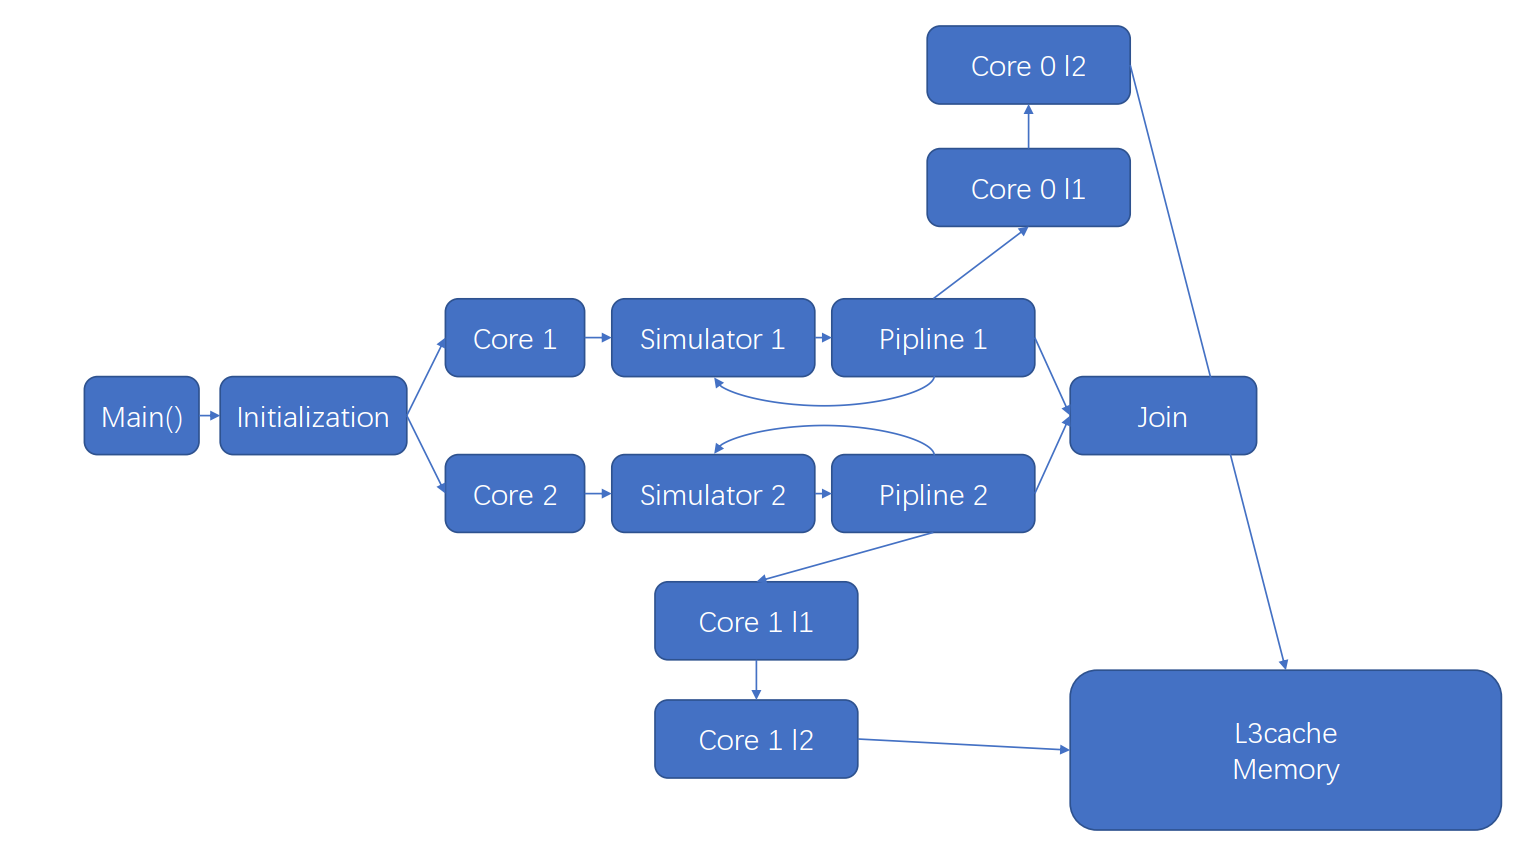
\includegraphics[scale = 0.28]{7.png}
\end{center}


\subsection{Test and Correctness}
To test task1, you should input format string at ternimal which I mentioned in preknowledge before. It is simply to test whether it is correct since the platform has already offer some .riscv file. And I'll put several results as pictures bellow, you can also choose your test file.\\
Notice, since the output is too long, I part it into several pictures.\\
This is test for \textbf{matrixmulti.riscv} and \textbf{quicksort.riscv}:\\
\begin{center}
  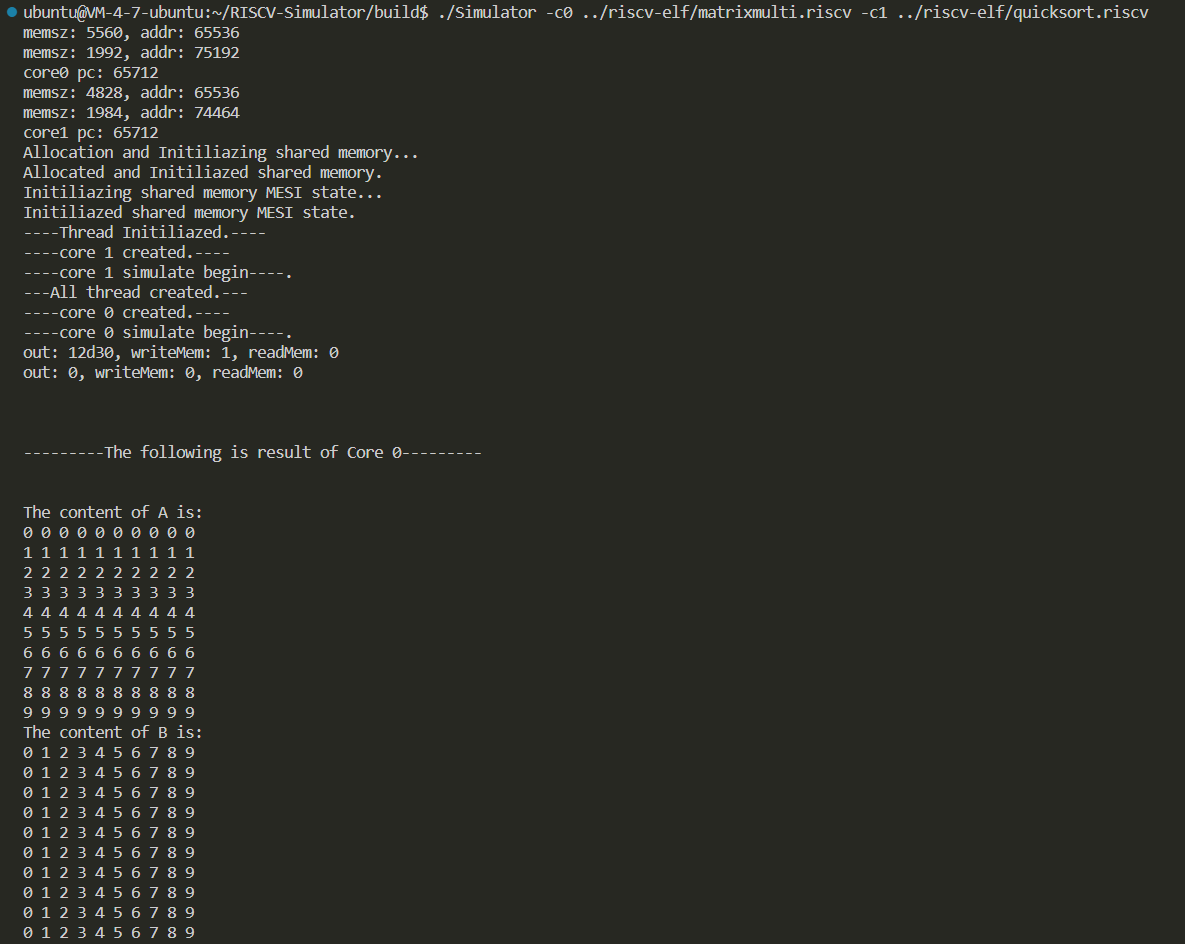
\includegraphics[scale = 0.3]{1.png}
  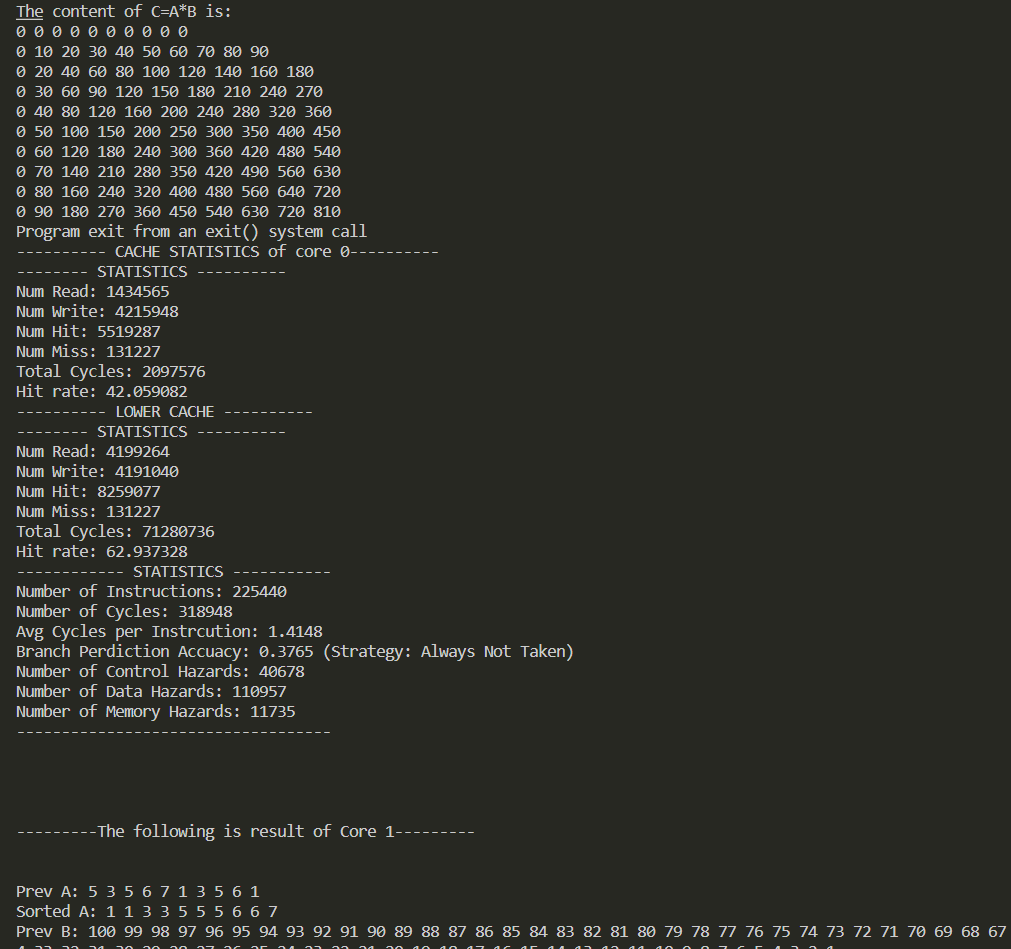
\includegraphics[scale = 0.3]{2.png}
  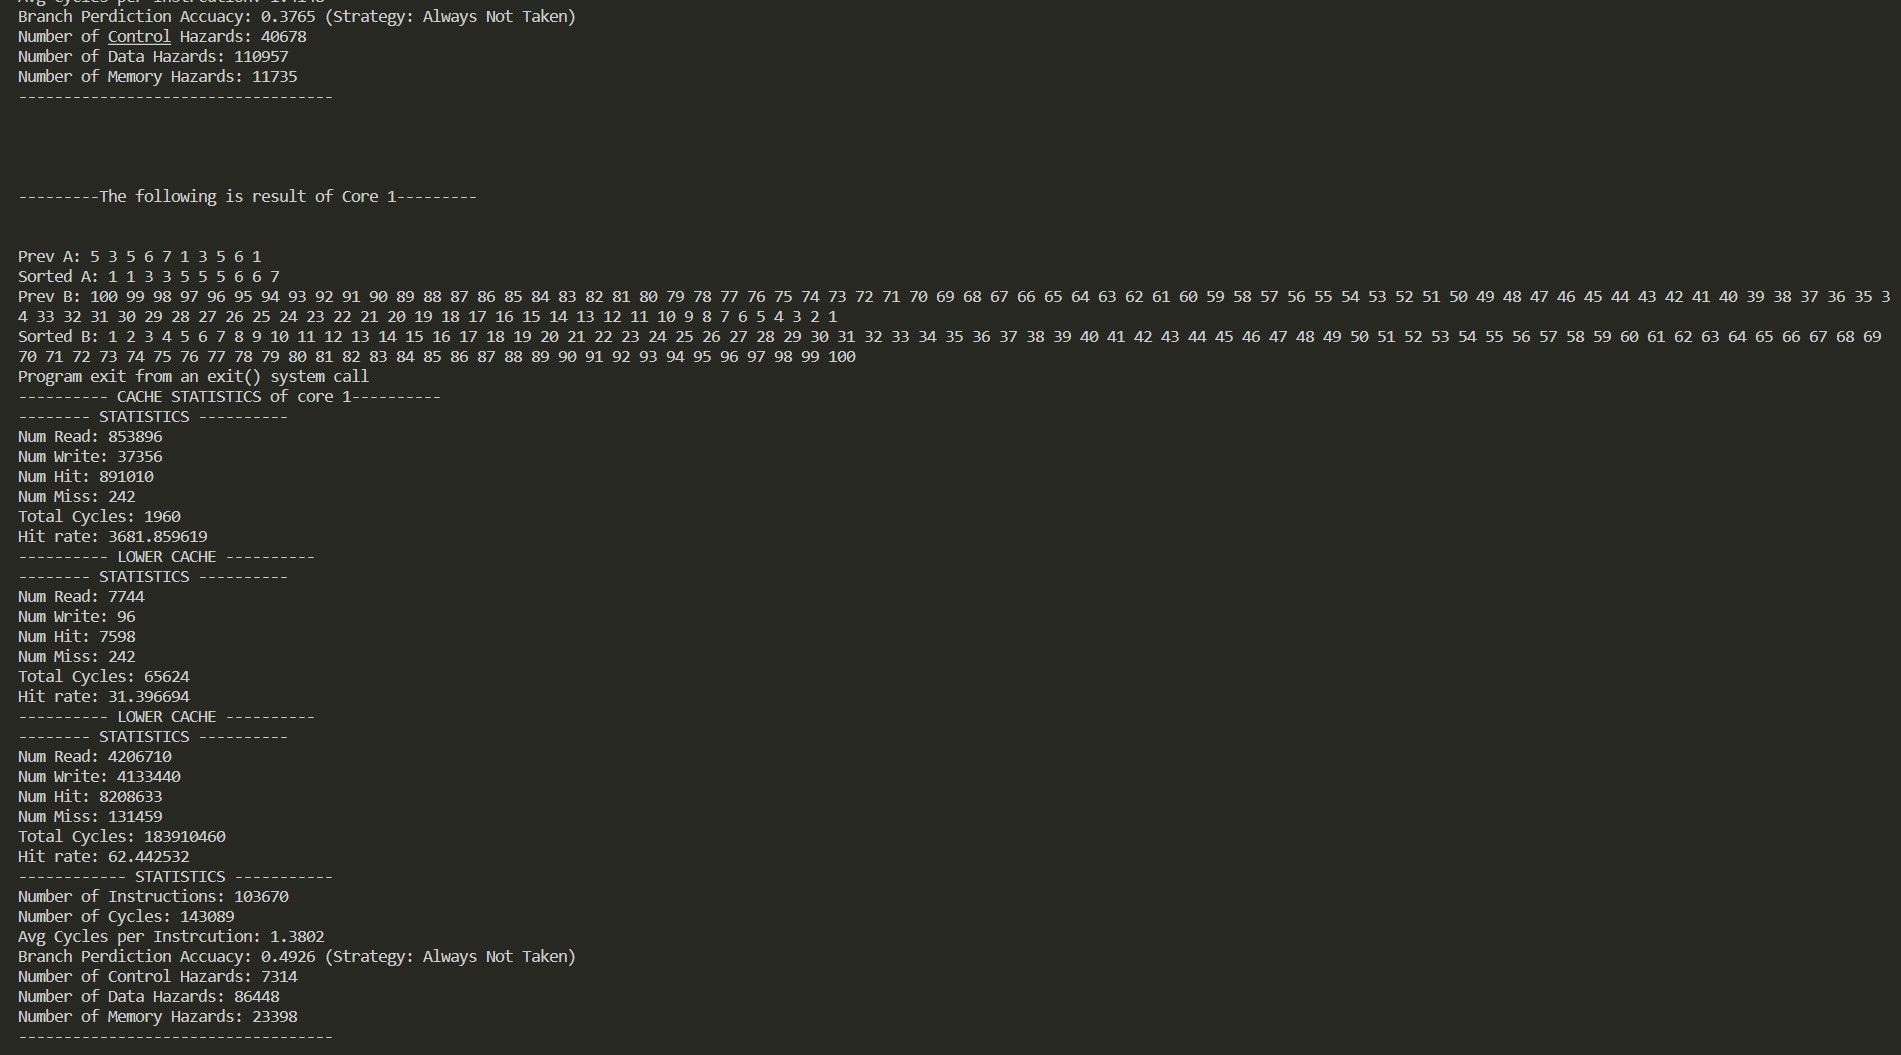
\includegraphics[scale = 0.25]{3.png}
\end{center}
This is test for \textbf{ackermann.riscv} and \textbf{matrixmulti.riscv}:\\
\begin{center}
  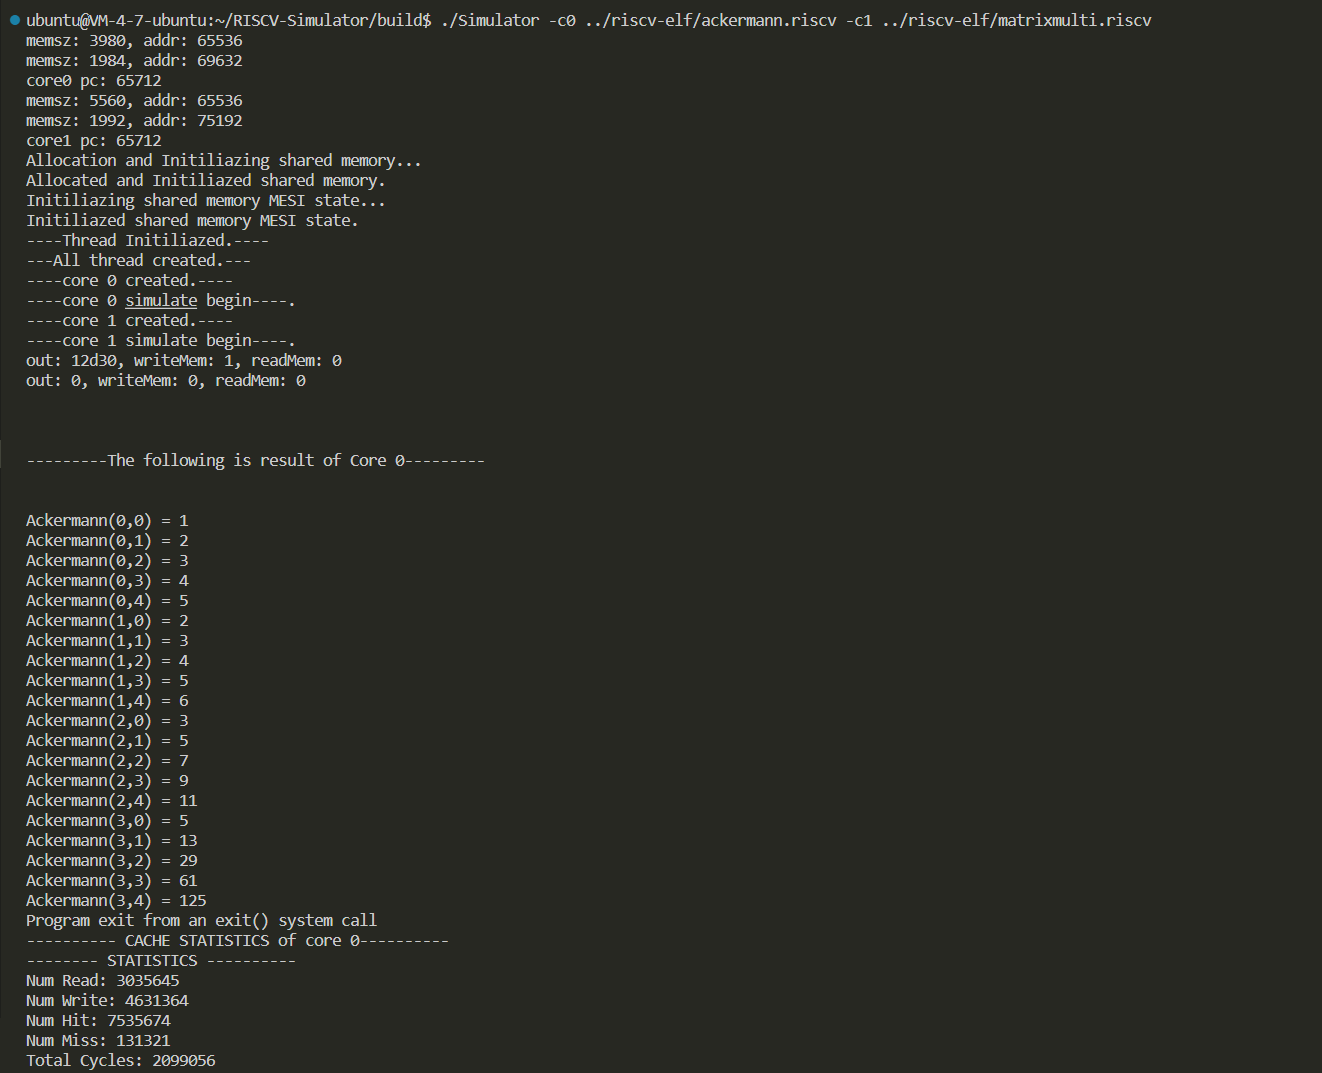
\includegraphics[scale = 0.28]{4.png}
  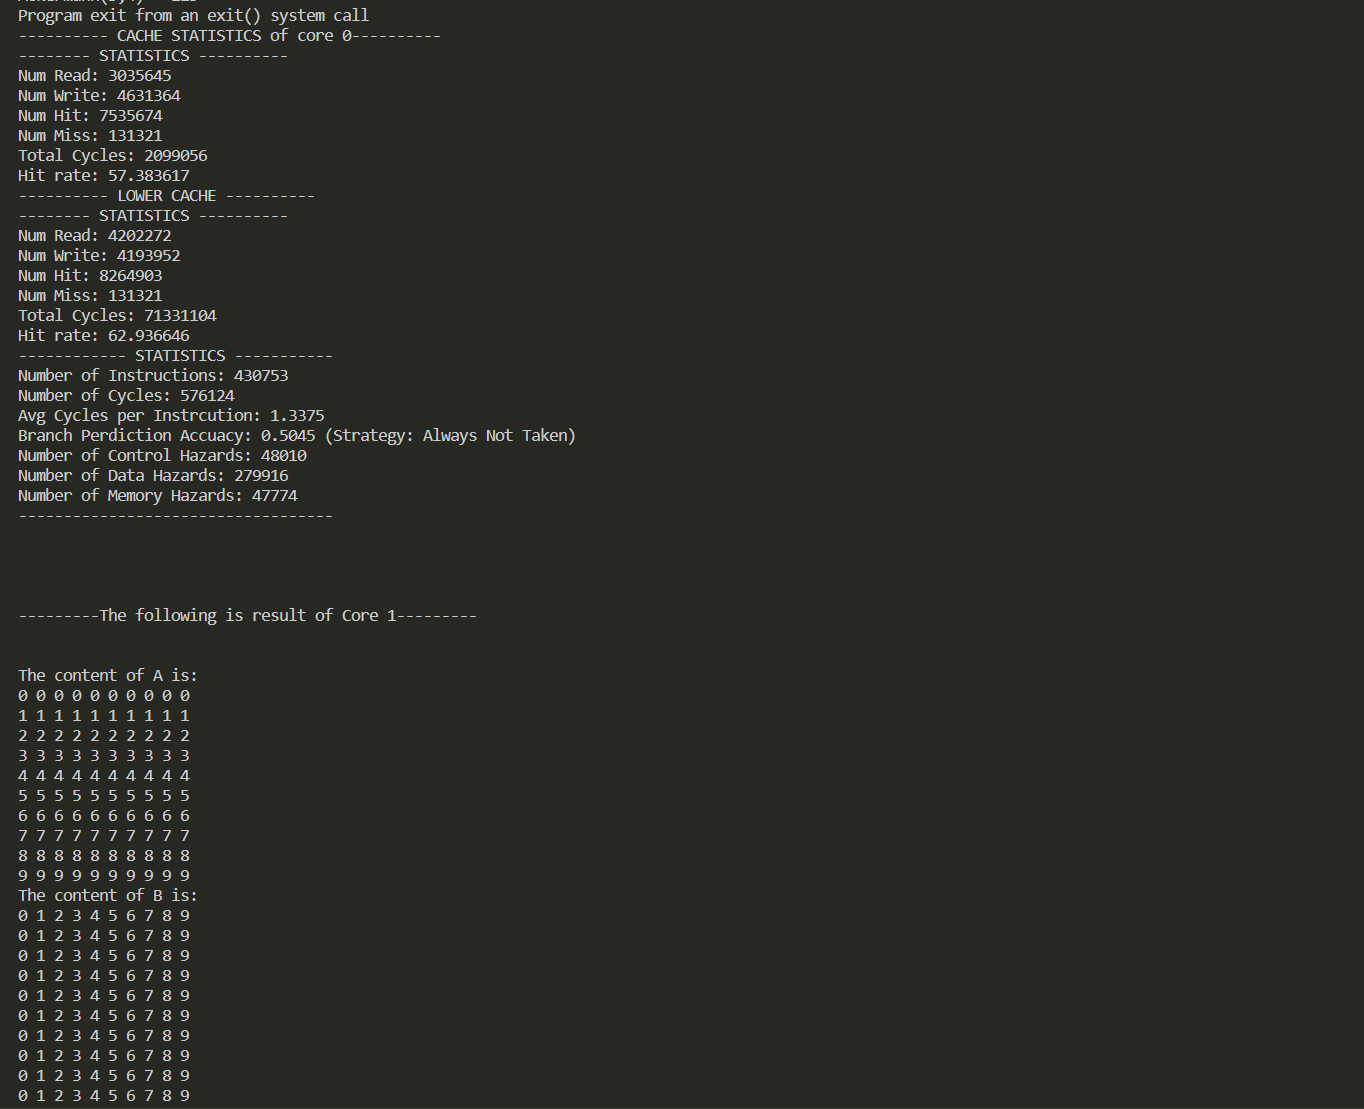
\includegraphics[scale = 0.3]{5.png}
  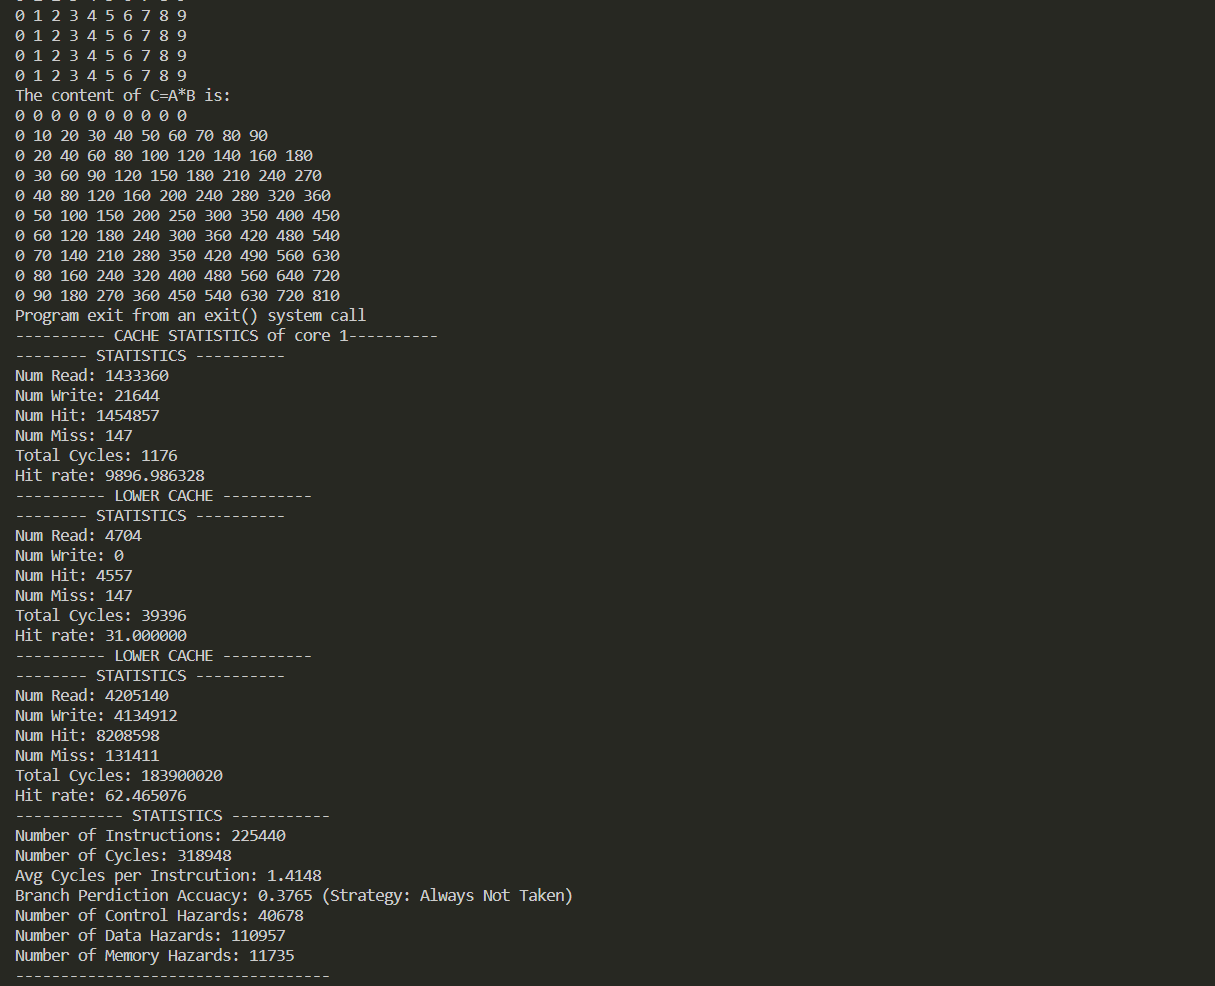
\includegraphics[scale = 0.3]{6.png}
\end{center}
As I mentioned before, the reason why the output is so "beautiful" is because I hold the output of different thread into specified string buffer, it will look very ugly without this method multi thread ouput :(.\\
We can see that the program run currently and print current result.

\section{Task2}
\subsection{Requirement}
\begin{itemize}
  \item Realize MESI based on directories. 
  \item Running two official test programs, add false sharing tests, verify implementation
  \item Bonus for same cache line same cycle memory operation.
\end{itemize} 

\subsection{Implementation}
\subsubsection{Shared Memory}
Since the test programs ask for 4MB shared memory from $0x100000$ to $0x500000$, I choose this space as default shared memory space and allocate it at the begining of this simulator, the address in this area will not influenced by B\&B policy and will handled by MESI directory. All other memory space will keep the same as no MESI policy.\\
Each time when we try to operate on shared memory, we will first try to get a lock \textbf{l3cache\_mainmemory\_lock} which declared in \textbf{MainCPU.cpp} and externed in \textbf{Cache.cpp} to avoid operate on the same cache, though it is inefficient , can fullfill complex multithread running environment well. 
\subsubsection{MESI}
We first affirm that it is private l1, l2 cache, shared l3 cache. The policy is write back and write allocate.\\
Normally, directory based on MESI are like this, cache line has 4 status: \textbf{C-invalid}, \textbf{C-shared}, \textbf{C-modified}, \textbf{C-transient}, memory line has 4 status: \textbf{R(dir)}, \textbf{W(id)}, \textbf{TR(dir)}, \textbf{TW(id)}. However, in software implementation, memory operation should finished all together in one instruction, and it should have \textbf{E} state. To simplify, each level of each core cache will have a bit to store it's state, including shared l3 cache, also memory will have a bit to store its state. So I finally set my MESI directory as follows
\begin{lstlisting}[language=c++]
/* MESI cacheline state */
enum cache_state
{
  CM = 0, /* Modified, should be the only one among all cache, memory */
  CE = 1, /* Exclusive, only owned by one core */
  CS = 2, /* Shared, have multiple copy among different core, memory */
  CI = 3, /* Invalid */
  CN = 4, /* Initialize State, for debug, it should be same as CI */
};
  
/* MESI memory line state */
enum memory_state
{
  MS = 0, /* Shared, valid data */
  MI = 1, /* Invalid */

/* MESI directory */
cache_state share_memory_cache[SHARE_CACHELINE_SIZE][2][3];
memory_state share_memory_memory[SHARE_CACHELINE_SIZE];
};
\end{lstlisting}
For initilization, all shared memory line are set to \textbf{MS}, all shared cache line are set to \textbf{CN}. \\
For shared memory space read:(suppose current is core 0)
\begin{itemize}
  \item If core 0 cache hit, then all directory state keep the same.
  \item If core 0 cache miss, enter into memory, see for directory.
    \begin{itemize}
      \item If memory data state is MS(shared), read data back.
        \begin{itemize}
          \item If the data is only shared in memory, then core 0 l1, l2, l3 are all CE.
          \item If the data has other valid copy in core 1, then core 0 l1, l2, l3 are all CS.
        \end{itemize}
      \item If memory data state is MI(in another core), find the data in another core(it is sure that the first hit in another core is the right copy), read back to memory, set another core data state to be CS, set memory state to MS. Read back to core 0, and set state to CS. 
    \end{itemize}
\end{itemize} 
For shared memory space write:(suppose current is core 0), since it is write allocate, we first make sure that the right copy should appear in core 0 l1 cache.
\begin{itemize}
  \item If core 0 l1 cache has valid copy, write into it, and see other state
    \begin{itemize}
      \item If previous core 0 l1 cache state is CE, set it to CM, invalid any valid copy in core 0 space(core 0 l2, shared l3, memory) if they have, set their cache line valid bit to invalid, and state to MI
      \item If previous core 0 l1 cache state is CS, set it to CM, invalid any valid copy in other space(core 0 l2, core 1 l1, l2, shared l3, memory) if they have, set their cache line valid bit to invalid, and state to MI
      \item If previous core 0 l1 cache state is CM, do nothing.
    \end{itemize}
  \item If core 0 l1 cache do not have valid copy, first read it, make sure that it has a valid copy in l1 cache, and see other state
    \begin{itemize}
      \item If previous core 0 l1 cache state is CE, set it to CM, invalid any valid copy in core 0 space(core 0 l2, shared l3, memory) if they have, set their cache line valid bit to invalid, and state to MI
      \item If previous core 0 l1 cache state is CS, set it to CM, invalid any valid copy in other space(core 0 l2, core 1 l1, l2, shared l3, memory) if they have, set their cache line valid bit to invalid, and state to MI
      \item If previous core 0 l1 cache state is CM, do nothing.
    \end{itemize}
\end{itemize}
For evicted policy, we know that a shared data need to be additional concerned if and only if its state is CM(since unmodified data copy wont write back)
\begin{itemize}
  \item If evit from shared l3 cache to memory, delete the state in l3 cache, write data back to memory, set memory state to MS.
  \item If evit from private cache, delete the state in the previous level cache, update in the next level cache.
\end{itemize}
The real implementation is quite complex and it is impossible to list here, I nearly add 2000 lines of code to write and test this. The comments is readable and please directly read the code.
\subsubsection{Additional Consider}
First there is the same situation with Lab1, the platform previous load or store data per byte(e.t. read a int will cause 4 read of bytes), more seriously, this will cause if one byte of data is write or read, it will change the cache/memory MESI state and then remain bytes of data will get a different state situation. To solve this, I support \textbf{CM} state data update all block directly back to memory. Thus, when the read int request to invalid memory is received, the first byte will update memory with the right core copy, and then the remain byte will get a valid memory copy, which do not harm to data correctness.\\
What's more, a write through cache will be more simple and easier to implemented, it actually used to be my choice but more inefficiency. So I finally to choose write allocate.\\ 
\subsection{Test and Correctness}
\subsubsection{True Sharing}
I directly run the official code, since the cache line size is 32.
First we test the correctness, I run several times with following command \textbf{./Simulator -c0 ../riscv-elf/lab3-core0.riscv -c1 ../riscv-elf/lab3-core1.riscv}, it have and should have three kinds of output:\\
core 0: S   core 1: C  
\begin{center}
  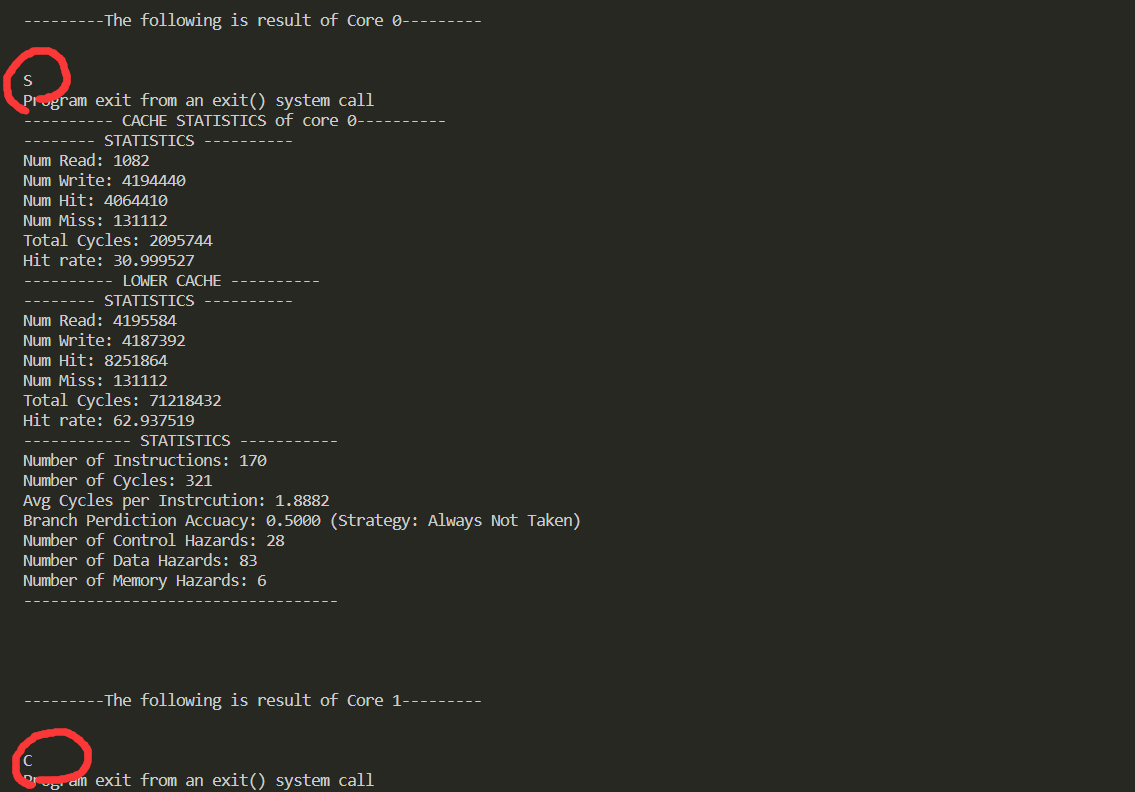
\includegraphics[scale = 0.2]{8.png}
\end{center}
core 0: S   core 1:(nothing)
\begin{center}
  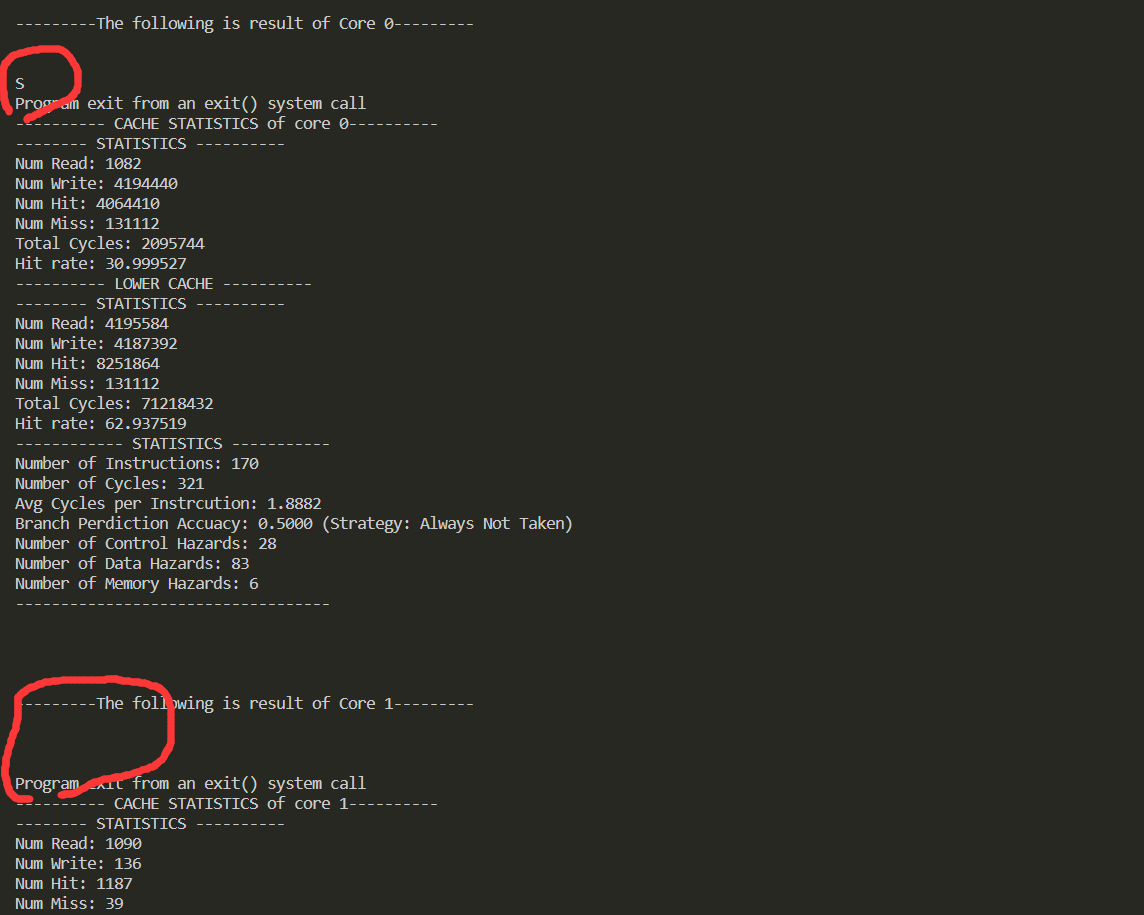
\includegraphics[scale = 0.2]{9.png}
\end{center}
core 0:(nothing)   core 1:C
\begin{center}
  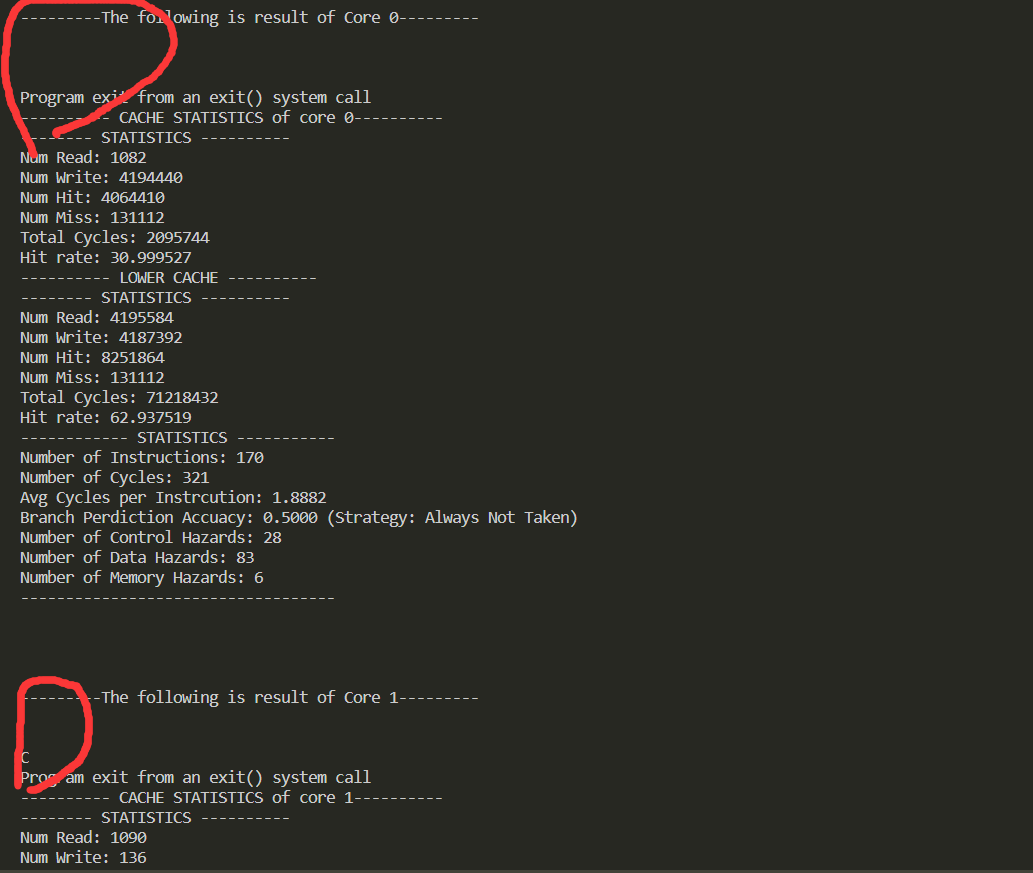
\includegraphics[scale = 0.2]{10.png}
\end{center}
Next, we use the debug ouput to make sure that it is true sharing. For example, suppose two core all write data before each other read, \textbf{lab3-core1.c} modified a[257], thus when \textbf{lab3-core0.c} read a[257], it will find invalid in memory and copy data back from core 1.\\
Here is what \textbf{lab3-core1.c} write a[257] happen:
\begin{center}
  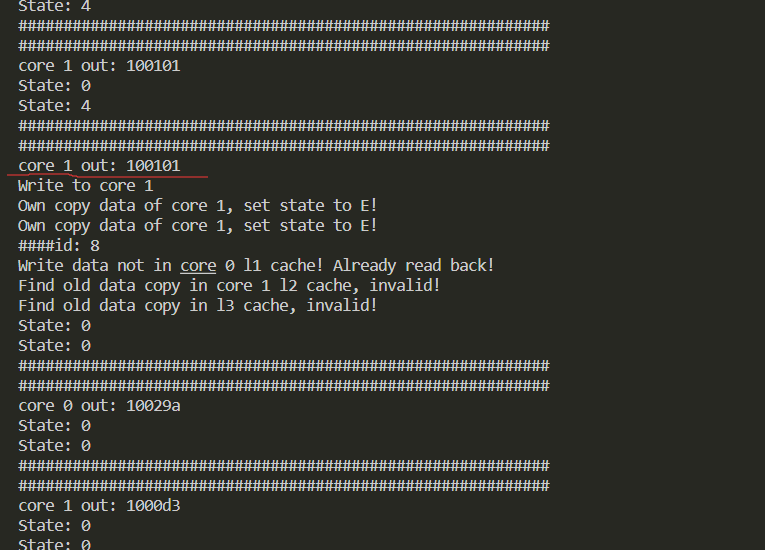
\includegraphics[scale = 0.4]{11.png}
\end{center}
We can see that when core 1 write, core 1 has valid copy in core 1 l1 cache, and the copy in core 1 l2 cache, shared l3 cache, memory are all invalid. Then, when core 0 try to read it:
\begin{center}
  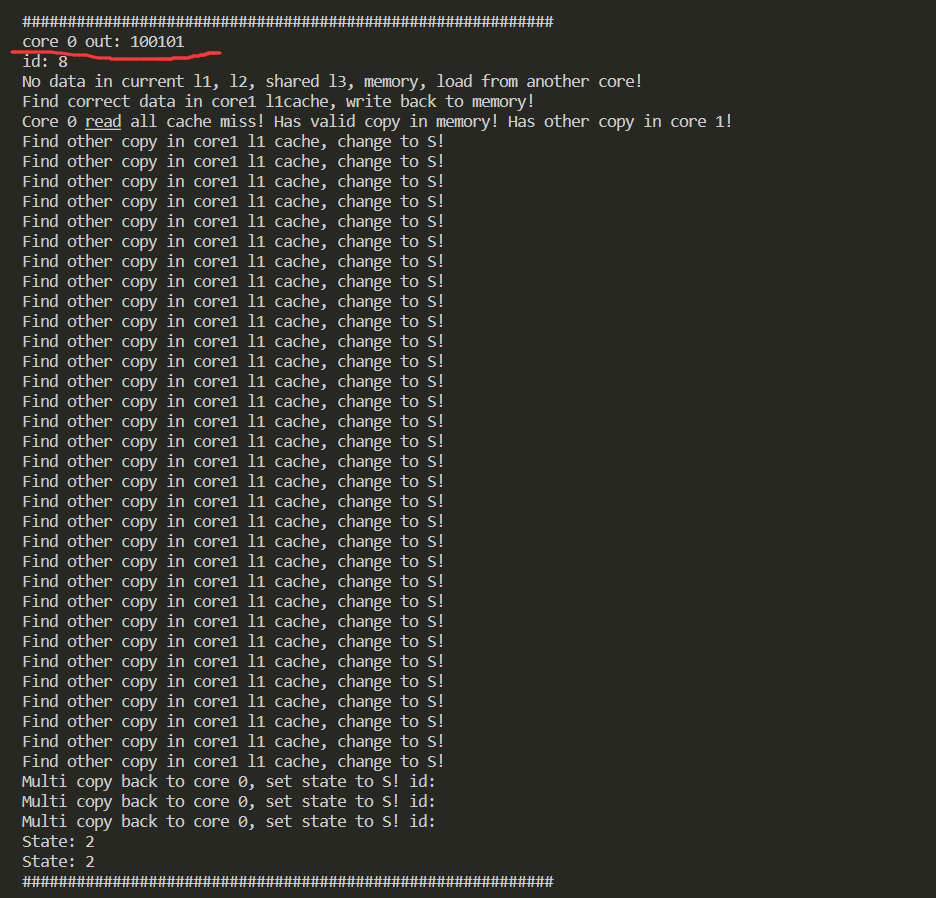
\includegraphics[scale = 0.4]{12.png}
\end{center}
We can see that when core 0 read, it find that the copy in memory is invalid, the request let core 1 write data back to memory. Then core 0 read it back and set state to S. Thus, we proved that the true sharing situation is correct.
\subsubsection{Fasle Sharing}
I run two programs write by myself. \textbf{lab3-core0-test1.c} multiple write to array \textbf{a} from index 0 to index 9, and \textbf{lab3-core1-test1.c} multiple write to array \textbf{a} from index 10 to index 19(this two programs and corresponding .riscv can be found in ./test and ./riscv-elf). We know that they do not write each other's memory space, after the first write of each other, they should not occur any write miss. Since the multi thread might execute dynamic code in different oder, so here is just a example show that they actually suffer from write miss,
\begin{center}
  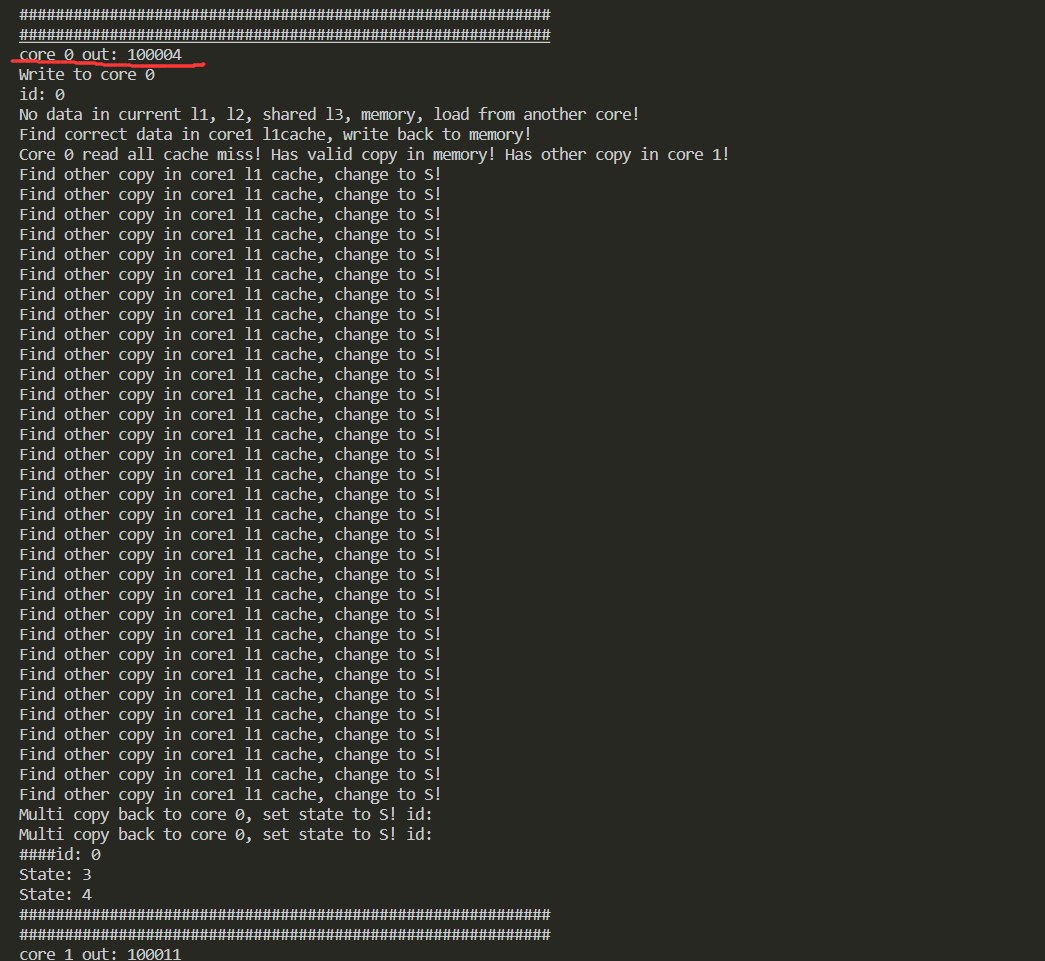
\includegraphics[scale = 0.4]{13.png}
\end{center}
As show in the picture, when core 0 try to write a[4], it suffer a write miss which caused by core 1 right, since all the write are in a same cache line, which is called a false sharing. Thus, proved that false sharing is right.
\subsection{How to deal with writing to same cache line conflict?}
It is quite hard to implemented a totally parallel program that run on two cores, the cache structure is quite urgly. As you can see before, for code which not used shared memory, I allow them to execute paralleled, for code which used shared memory, I'll check and let them execute in sequential.

\section{Something Want to Tell}
Dear TA,\\
Hello,\\
This is a note that when I finished all labs I want to leave to you, this RISCV-Simulator is actually not a very good simulator platform.\\
There are some reasons,\\
First, the cache hit rate calculation is wrong, since the author implement cache as once a time load a byte no matter it is a int request or a long int request, which results the first byte read the whole cache line into cache, and the remaining bytes are all cache hit! Thus, for example, when I once read a int data, I got only one cache miss and three cache hit! Is this real in life to calulate a cache hit rate?\\
Second, also about the cache, the author use highly resursion structure to implement multi level cache. It violate engineering code specification, since its compatibility is quite low and easy to broken down when try to modified it. Also, it is quite strange about its program flow design, the class MemoryManager both handle cache and memory(but actually author design to let MemoryManager just be main memory). That means student have to pay a lot time to understand how the author implement simple concept taught in class and try to obey its strange design. This semester I also choose Operating System, the project is writing a naive system called PintOS, I feel there is indeed a significant gap in engineering quality between the two source codes.\\
Third, actually when I talked with the author of this platfrom(I pose a PR to fix a bug of the Simulator before), it is just a curriculum design and there might exist several bugs or even design discount. I'm also wondering if there is a better Simulator you can use in the next few years.\\
I understand the lab is aim to practise what we learned in class, but I just feel that I spend a little more time on something not related with this target. There might not exist a better one, or I guess Prof. Wang are aim to training our ability of reading and modifying "Shit Mountain". Anyway, it just something I want to tell you, and I hope that the Simulator will be improved in the next few years. This course is a nice course, and teach me a lesson that Prof. Wang has said many times, "Simple, but not easy." 

\end{document}
